\documentclass[12pt]{article}\usepackage[]{graphicx}\usepackage[dvipsnames]{xcolor}
% maxwidth is the original width if it is less than linewidth
% otherwise use linewidth (to make sure the graphics do not exceed the margin)
\makeatletter
\def\maxwidth{ %
  \ifdim\Gin@nat@width>\linewidth
    \linewidth
  \else
    \Gin@nat@width
  \fi
}
\makeatother

\definecolor{fgcolor}{rgb}{0.345, 0.345, 0.345}
\newcommand{\hlnum}[1]{\textcolor[rgb]{0.686,0.059,0.569}{#1}}%
\newcommand{\hlstr}[1]{\textcolor[rgb]{0.192,0.494,0.8}{#1}}%
\newcommand{\hlcom}[1]{\textcolor[rgb]{0.678,0.584,0.686}{\textit{#1}}}%
\newcommand{\hlopt}[1]{\textcolor[rgb]{0,0,0}{#1}}%
\newcommand{\hlstd}[1]{\textcolor[rgb]{0.345,0.345,0.345}{#1}}%
\newcommand{\hlkwa}[1]{\textcolor[rgb]{0.161,0.373,0.58}{\textbf{#1}}}%
\newcommand{\hlkwb}[1]{\textcolor[rgb]{0.69,0.353,0.396}{#1}}%
\newcommand{\hlkwc}[1]{\textcolor[rgb]{0.333,0.667,0.333}{#1}}%
\newcommand{\hlkwd}[1]{\textcolor[rgb]{0.737,0.353,0.396}{\textbf{#1}}}%
\let\hlipl\hlkwb

\usepackage{framed}
\makeatletter
\newenvironment{kframe}{%
 \def\at@end@of@kframe{}%
 \ifinner\ifhmode%
  \def\at@end@of@kframe{\end{minipage}}%
  \begin{minipage}{\columnwidth}%
 \fi\fi%
 \def\FrameCommand##1{\hskip\@totalleftmargin \hskip-\fboxsep
 \colorbox{shadecolor}{##1}\hskip-\fboxsep
     % There is no \\@totalrightmargin, so:
     \hskip-\linewidth \hskip-\@totalleftmargin \hskip\columnwidth}%
 \MakeFramed {\advance\hsize-\width
   \@totalleftmargin\z@ \linewidth\hsize
   \@setminipage}}%
 {\par\unskip\endMakeFramed%
 \at@end@of@kframe}
\makeatother

\definecolor{shadecolor}{rgb}{.97, .97, .97}
\definecolor{messagecolor}{rgb}{0, 0, 0}
\definecolor{warningcolor}{rgb}{1, 0, 1}
\definecolor{errorcolor}{rgb}{1, 0, 0}
\newenvironment{knitrout}{}{} % an empty environment to be redefined in TeX

\usepackage{alltt}
\usepackage{amsmath,amsfonts,amssymb,graphicx,authblk}
\usepackage[font={footnotesize,singlespacing},labelfont=bf]{caption}
\usepackage{titlesec,blkarray, bm} 
\usepackage{float,afterpage}
\usepackage[running,mathlines]{lineno}
\usepackage[vmargin=1in,hmargin=1in]{geometry}
\usepackage[authoryear,sort]{natbib}
\usepackage[dvipsnames]{xcolor}
\usepackage[nodisplayskipstretch]{setspace} 
\usepackage{hyperref}
\usepackage[section]{placeins}
\usepackage{gensymb}
\usepackage{enumitem}
\usepackage{orcidlink}
\setlist{topsep=.125em,itemsep=-0.15em,leftmargin=0.75cm}
\setlength{\parindent}{0.35in}

\usepackage[sc]{mathpazo} %Like Palatino with extensive math support
\usepackage[subtle]{savetrees}

\usepackage{lineno}
%\renewcommand{\refname}{Literature Cited}
%\renewcommand{\floatpagefraction}{0.9}
%\renewcommand{\topfraction}{0.99}
%\renewcommand{\textfraction}{0.05}

\clubpenalty = 10000
\widowpenalty = 10000

\sloppy 

\usepackage{ifpdf}
\ifpdf
\DeclareGraphicsExtensions{.pdf,.png,.jpg}
\usepackage{epstopdf}
\else
\DeclareGraphicsExtensions{.eps}
\fi

\graphicspath{{/Users/jm200/Library/CloudStorage/Dropbox/Miller Lab/github/ELVI-endophyte-density/Figure/}}
\newcommand{\tom}[2]{{\color{red}{#1}}\footnote{\textit{\color{red}{#2}}}}
\newcommand{\jacob}[2]{{\color{blue}{#1}}\footnote{\textit{\color{blue}{#2}}}}
%\doublespacing



% I cannot get \orcidlink working on my computer so for now replacing this with \textit

%-------------------------------------------------------------------------
\title{Effect of grass-endophyte symbiosis and herbivory on population demography across a climatic and geographic gradient}
\author[1]{Jacob K. Moutouama\,\textit{0000-0003-1599-1671} \thanks{Corresponding author: jmoutouama@gmail.com}}
\author[1]{Julia Martin}
\author[1]{Ulisses Rizo}
\author[1]{Malcolm Sherwood}
\author[1]{Emily Chong}
\author[1]{Dajanae Pearson}
\author[1]{Alexandra Jimenez Martín}
\author[2]{Josh Fowler}
\author[1]{Ali Campbell}
\author[1]{Chris Oxley}
\author[1]{Karl Schrader}
\author[1]{Tom E.X. Miller\,\textit{0000-0003-3208-6067}}
\affil[1]{Program in Ecology and Evolutionary Biology, Department of BioSciences, Rice University, Houston, TX USA}
\affil[2]{University of Miami, Department of Biology, Miami, FL USA}
\date{} % clear date
%\renewcommand\Authands{ and }

\sloppy

%-------------------------------------------------------------------------
\IfFileExists{upquote.sty}{\usepackage{upquote}}{}
\begin{document}
%\SweaveOpts{concordance=TRUE}
\renewcommand{\baselinestretch}{1.2}
\maketitle
% \bigskip 
%45 character limit on running head
\noindent\textbf{Running header:} Grass-endophyte-herbivory effects across gradients
\bigskip 

\noindent\textbf{Keywords:} demography, range limits

\bigskip 
\noindent\textbf{Submitted to:} \textit{Ecology letters} (Letter)

\bigskip 
\noindent\textbf{Data accessibility statement:} 
If the paper is accepted, all data and computer scripts supporting the results will be archived in a Zenodo package, with the DOI included at the end of the article. 
During peer review, our code (Stan and R) is available at \url{https://github.com/jmoutouama/ELVI-endophyte-density}. 

\bigskip 
\noindent\textbf{Conflict of interest statement:} None.

\bigskip
\noindent\textbf{Authorship statement:}
%J.K.M., A.C. and T.E.X.M. designed the study.
%A.C. and T.E.X.M. collected the data. 
%All authors conducted the statistical analyses and modeling.
%J.K.M. drafted the manuscript, and T.E.X.M contributed to revisions.

\bigskip
\noindent\textbf{Abstract:}\\
\noindent\textbf{Main Text:}\\
\noindent\textbf{Figures: 6}\\
\noindent\textbf{Tables: X}\\
\noindent\textbf{References: X}

\newpage
%\SweaveOpts{concordance=TRUE}
\linenumbers
%-------------------------------------------------------------------------
\spacing{1.25}
\section*{Abstract}
%150 words limit for Ecology letter. The number now is 
Interactions between plants and fungi are ubiquitous in nature and have significant effects on plant fitness.
However, the extent to which variation in fungal frequency affects plant distribution remains understudied. 
Using three cool-season grass species, we combined field experiments on plant populations with variation in leaf endophytic fungi and Bayesian statistics to test whether plant-fungi interactions constrain host demography and, consequently, geographic range limits. 
We found that all vital rates decreased toward the species' range edges, indicating reduced demographic performance in these regions. 
This decline was more pronounced in individuals hosting endophytic symbionts, suggesting that plant-fungi interactions that are beneficial under benign conditions may become parasitic under stressful conditions.
Our results highlight that range expansion may be hindered by the presence of a mutualist.

%--------------------------------------------------------------------
\newpage
\section*{Introduction}
Plant-microbe symbioses are widespread and ecologically important. 
These interactions are famously context-dependent, where the direction and strength of the interaction outcome depends on the environment in which it occurs \citep{fowler2023geographic,hoeksema2015context, bronstein1994conditional}.
Plant-microbe  interactions that are beneficial under stressful conditions  may become parasitic under benign conditions \citep{giauque2019endophyte}.
Under biotic stress (e.g., herbivory), endophyte symbiosis can benefit host plants by facilitating the production of secondary compounds that deter feeding or exert direct toxicity, thereby reducing insect growth, survival, and oviposition \citep{atala2022fungal,bastias2017epichloe,vega2008insect}.
Similarly under abiotic stress (e.g., drought), symbionts can increase their host tolerance  \citep{clay2002evolutionary}.
However, in many plant-microbe interactions, host protection is not guaranteed solely by the presence of a symbionts; rather, the density of the symbiont can determine the effectiveness of this protection \citep{laughton2014combined}. 
Higher endophyte densities may lead to increased resource exploitation by the symbiont, potentially imposing costs on the host, such as reduced growth or reproduction \citep{faeth2009asexual}.
%This cost is often manifested by a reduction in host biomass or reproductive success \citep{faeth2009asexual}, particularly under harsh abiotic conditions \citep{cui2024review}. 
%Ultimately, these context-dependent costs and benefits may underlie the observed distribution of host species.

Context dependence raises the hypothesis that plant-microbe interactions are likely to vary across environmental gradients, from range core to range edge, with significant implications for host range expansion. If microbial symbiosis provides greater benefits under environmental stress, then symbionts could enhance the suitability of range-edge environments, potentially extending host range limits \citep{allsup2023shifting,rudgers2020climate}.
For instance, fungal endophytes improve the survival of \emph{Bromus laevipes}  populations in dry conditions, increasing their drought resistance at the range edge and thereby extending the species' geographic range \citep{david2019soil,afkhami2014mutualist}.
Even if the symbiont does not directly improve host survival, it may still enhance host population growth over time by increasing relative growth and reproduction, potentially offsetting the negative effects of lower survival rates \citep{yule2013costs}.
Conversely, if microbial symbiosis is costly for the host at range edge, symbionts could constrain host range \citep{benning2021microbes,benning2021plant,bennett2022costs}.
%Mutualist limitation reduces population fitness and therefore limits range expansion in \emph{Medicago polymorpha} populations \citep{lopez2021microbial}. 
%Although context dependence, along with spatiotemporal variations in abiotic environmental conditions may reduce the effectiveness of the benefits provided by the symbiont to the host species, our understanding of the mechanisms that alter host-symbiont interactions across species geographic range remains limited.

Despite growing interest in the ecological and evolutionary roles of symbiosis, most studies focus on the host plant’s perspective and rarely manipulate symbiont prevalence to evaluate how environmental variation shapes the symbiont’s effects on host demography across geographic ranges. 
Yet, symbionts promote their own fitness by influencing host life history traits and enhancing resistance to stress \citep{kazenel2015mutualistic, giauque2019endophyte, saikkonen1998fungal}. 
Theory predicts that exclusive vertical transmission fosters mutualism and leads to high symbiont prevalence in host populations \citep{fine1975vectors}. 
Field studies suggest that, under stressful conditions, beneficial symbionts may increase in prevalence and even reach fixation if their fitness advantages outweigh reproductive costs \citep{donald2021context}. 
However, populations with lower prevalence may experience higher symbiont loss among offspring \citep{afkhami2008symbiosis}. 
Thus, overlooking symbiont dynamics could result in incomplete predictions of host population responses to global change.

Additionally, few studies address the synergistic effects of abiotic and biotic stressors on host-symbiont dynamics across species’ ranges.
For example, herbivory not only affects the fitness benefits of symbiosis but can also increase endophyte prevalence through enhanced vertical transmission \citep{gundel2020simulated, agrawal1999transgenerational}.
However, these findings are primarily based on greenhouse studies, which limits our understanding of how herbivory shapes natural population dynamics, especially under variable field conditions.
If the ecological context in which herbivory occurs alters plant fitness, then interactions between herbivory and abiotic stress (e.g., drought) may substantially influence population dynamics and species range  limitation.

Working across a precipitation gradient in the south-central US, we investigated  how the demographic effects of endophyte symbiosis vary from core to edge of the host range.
To answer that question, we studied the symbiotic association between cool-season grass species (\emph{Agrostis hyemalis}, \emph{Elymus virginicus} and \emph{Poa autumnalis}) and their  vertically transmitted fungal symbiont \emph{Epichloë} spp. 
Our experiment was design to test the following hypotheses:
\begin{enumerate}
    \item Stress associated with aridity and low precipitation enhances plant–fungal mutualism, such that the fitness benefits of endophyte symbiosis (survival, growth, and fecundity) are maximized at the range edge.
    \item Stress associated with herbivory weakens plant–fungal mutualism, such that the fitness costs of endophyte symbiosis (survival, growth, and fecundity) are maximized at the range edge.
\end{enumerate}
%--------------------------------------------------------------------
\section*{Materials and methods}
\subsection*{Study system}
Our study was conducted across seven sites along a geographic and climatic gradient spanning Louisiana and Texas in the United States (Fig.~\ref{fig:site}; Fig.\ref{sup:md}).  
At each site, we established eight plots (1.5 m $\times$ 1.5 m) containing individuals of three cool-season perennial grasses native to woodland and prairie habitats of eastern North America \citep{shaw2011guide}: \emph{Agrostis hyemalis}, \emph{Elymus virginicus}, and \emph{Poa autumnalis} (subfamily Pooideae).  
These species are capable of both self-pollination and outcrossing \citep{church1958artificial}.  
They typically host seed-transmitted fungal endophytes.
%however, \emph{Poa autumnalis} may also acquire endophytes via horizontal transmission \citep{gundel2020simulated}.
Seeds were collected in summer–fall 2006 from naturally symbiotic populations (source populations) of the three focal host species. These seeds were either heat-treated to eliminate symbionts or left untreated, thereby generating symbiont-free ($E^-$) and symbiotic ($E^+$) plants from the same genetic lineages as the source populations.

Across all sites, each plot was randomly assigned one of four initial endophyte frequency treatments (80\%, 60\%, 40\%, or 20\%) and one of two herbivory treatments (herbivore exclusion or herbivore access).  
We ensured that all plots received comparable quantities of source plant material.
This experimental design was informed by natural patterns of endophyte prevalence observed in Texas, where the proportion of symbiotic individuals has been reported as 86.55\% in \emph{A. hyemalis} (ranging from 77.16\% to 93.5\%) \citep{donald2021context}, 53\% in \emph{E. virginicus} (ranging from 10\% to 100\%) \citep{sneck2017variation}, and 96\% in \emph{P. autumnalis} \citep{rudgers2009fungus}.  
Additionally, fungal genotyping has confirmed the presence of biosynthetic pathways for secondary metabolites such as peramine, loline, and ergot alkaloids, which may enhance host resistance to drought and herbivory \citep{beaudry1951seed}.
Full details of the study design are provided in the supplementary materials.

\subsection*{Demographic data collection}
We collected demographic data including survival, growth, and reproduction in May and June of 2023 and 2024, which coincided with the flowering season of \emph{Agrostis hyemalis}, \emph{Elymus virginicus}, and \emph{Poa autumnalis}. 
For each individual, plant survival was recorded as a binary variable (alive or dead), and plant size was measured as the number of living tillers, indicated by the presence of green coloration.  
We recorded the number of inflorescences per plant and counted the number of spikelets on up to three inflorescences from three reproducing plants.  
Spikelet counts were limited to three reproducing tillers per plot due to the time-consuming nature of this measurement.  
We used the number of spikelets from these three tillers to estimate the average number of spikelets per plant.

\begin{figure}[H]
\centering
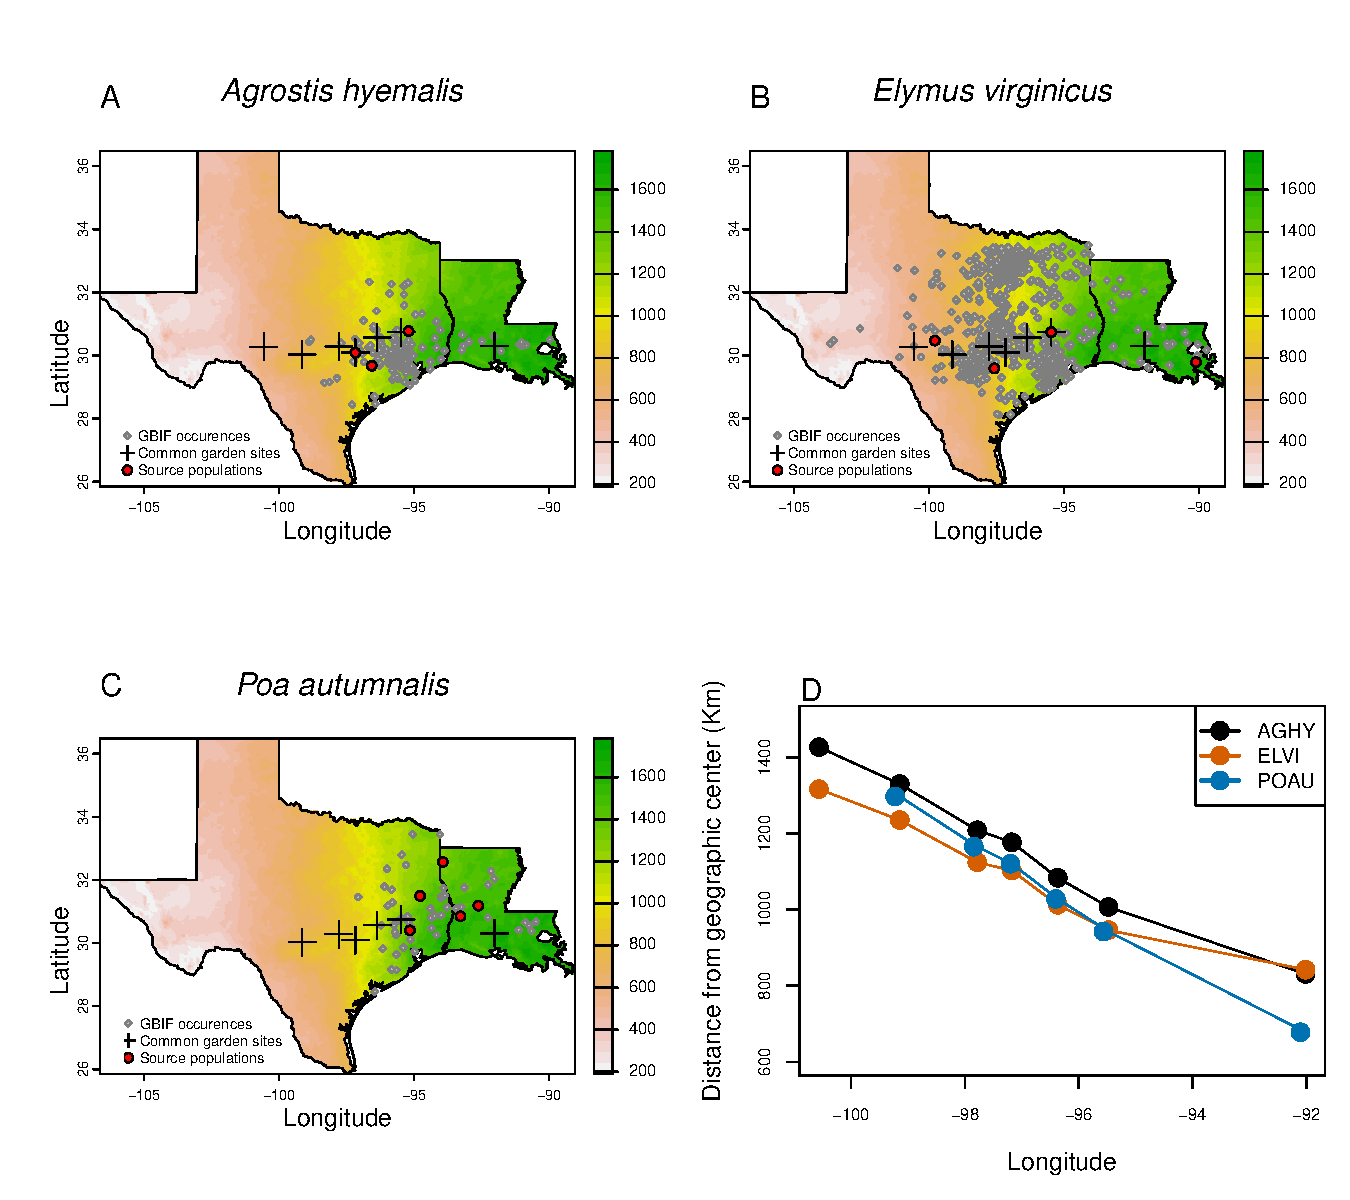
\includegraphics[width=1\textwidth]{clim_map1.pdf}
\caption{Distribution of common garden sites along the longitudinal aridity gradient in the central and southern Great Plains for: A) Agrostis hyemalis, B) Elymus virginicus, and C) Poa autumnalis. Red dots indicate the locations of source populations, while grey dots represent GBIF occurrence records for each species within the study area. D) Relationship between the distance from the range center and longitude for each species.}
\label{fig:site}
\end{figure}


\subsection*{Models building and models selection}
To assess how stress associated with aridity affects plant–fungal  interactions, we developed four candidate models for each vital rate (survival, growth, and fertility).  
Each vital rate was modeled using a grand mean intercept ($\beta_{0}$), slopes for variation in each covariate ($\beta_{1}$, $\beta_{2}$ and $\beta_{3}$), and interaction terms between covariates ($\beta_{4}$, $\beta_{5}$ and $\beta_{6}$).  
Each model included normally distributed random effects to account for site-to-site variation ($\phi \sim N(0,\ \sigma_{site})$), plot-to-plot variation ($\rho \sim N(0,\ \sigma_{plot})$), and source-to-source variation associated with the provenance of transplants used in the common garden ($\omega \sim N(0,\ \sigma_{source})$) (Eq.~\ref{eq:candidates}).

\begin{equation}\label{eq:candidates}
\begin{aligned}
\text{Model 1:} \quad 
\mu &= \beta_{0}^{\text{sp}} + \beta_{\text{P}}^{\text{sp}} P + \beta_{\text{endo}}^{\text{sp}}\,\text{endo} + \beta_{\text{herb}}^{\text{sp}}\,\text{herb} \\
&\quad + \beta_{\text{endo} \times \text{P}}^{\text{sp}}\,\text{endo} \cdot P 
+ \beta_{\text{herb} \times \text{endo}}^{\text{sp}}\,\text{herb} \cdot \text{endo} 
+ \beta_{\text{herb} \times \text{P}}^{\text{sp}}\,\text{herb} \cdot P \\
&\quad + \beta_{\text{P}^2}^{\text{sp}} P^2 + \beta_{\text{endo} \times \text{P}^2}^{\text{sp}}\,\text{endo} \cdot P^2 
+ \phi^{\text{sp}} + \omega^{\text{sp}} + \rho^{\text{sp}} \\
\text{Model 2:} \quad 
\mu &= \beta_{0}^{\text{sp}} + \beta_{\text{SPEI}}^{\text{sp}}\,\text{SPEI} + \beta_{\text{endo}}^{\text{sp}}\,\text{endo} + \beta_{\text{herb}}^{\text{sp}}\,\text{herb} \\
&\quad + \beta_{\text{endo} \times \text{SPEI}}^{\text{sp}}\,\text{endo} \cdot \text{SPEI} 
+ \beta_{\text{herb} \times \text{endo}}^{\text{sp}}\,\text{herb} \cdot \text{endo} 
+ \beta_{\text{herb} \times \text{SPEI}}^{\text{sp}}\,\text{herb} \cdot \text{SPEI} \\
&\quad + \beta_{\text{SPEI}^2}^{\text{sp}} \text{SPEI}^2 
+ \beta_{\text{endo} \times \text{SPEI}^2}^{\text{sp}}\,\text{endo} \cdot \text{SPEI}^2 
+ \phi^{\text{sp}} + \omega^{\text{sp}} + \rho^{\text{sp}} \\
\text{Model 3:} \quad 
\mu &= \beta_{0}^{\text{sp}} + \beta_{\text{GD}}^{\text{sp}}\,\text{GD} + \beta_{\text{endo}}^{\text{sp}}\,\text{endo} + \beta_{\text{herb}}^{\text{sp}}\,\text{herb} \\
&\quad + \beta_{\text{endo} \times \text{GD}}^{\text{sp}}\,\text{endo} \cdot \text{GD} 
+ \beta_{\text{herb} \times \text{endo}}^{\text{sp}}\,\text{herb} \cdot \text{endo} 
+ \beta_{\text{herb} \times \text{GD}}^{\text{sp}}\,\text{herb} \cdot \text{GD} \\
&\quad + \phi^{\text{sp}} + \omega^{\text{sp}} + \rho^{\text{sp}} \\
\text{Model 4:} \quad 
\mu &= \beta_{0}^{\text{sp}} + \beta_{\text{MD}}^{\text{sp}}\,\text{MD} + \beta_{\text{endo}}^{\text{sp}}\,\text{endo} + \beta_{\text{herb}}^{\text{sp}}\,\text{herb} \\
&\quad + \beta_{\text{endo} \times \text{MD}}^{\text{sp}}\,\text{endo} \cdot \text{MD} 
+ \beta_{\text{herb} \times \text{endo}}^{\text{sp}}\,\text{herb} \cdot \text{endo} 
+ \beta_{\text{herb} \times \text{MD}}^{\text{sp}}\,\text{herb} \cdot \text{MD} \\
&\quad + \phi^{\text{sp}} + \omega^{\text{sp}} + \rho^{\text{sp}}
\end{aligned}
\end{equation}

\noindent where \( sp \in \{1, 2, 3\} \) represents the species index, \( P \) denotes Precipitation, \( \text{SPEI} \) is the Standardized Precipitation Evapotranspiration Index, \( \text{GD} \) refers to distance from geographic center, and \( \text{MD} \) stands for mahalanobis distance, \( \text{endo} \) indicates Endophyte presence (binary), and \( \text{herb} \) represents Herbivory (binary). The terms \( \phi^{(sp)} \), \( \omega^{(sp)} \), and \( \rho^{(sp)} \) are plot-level, population-level, and site-level random effects, respectively, for species \( sp \).

Survival was modeled using a Bernoulli distribution, growth with a Gaussian distribution, flowering with a negative binomial distribution, and fertility (number of spikelets) also with a negative binomial distribution.
To assess the goodness-of-fit of the models, we performed posterior predictive checks \citep{gelman2000diagnostic, berkhof2000posterior}.  
All models effectively captured key aspects of the data, including means, standard deviations, and quantiles (Fig.~\ref{sup:ppc_surv}, Fig.~\ref{sup:ppc_growth}, Fig.~\ref{sup:ppc_spikelet}, Fig.~\ref{sup:ppc_flowering}).
To determine the best model for each vital rate, we compared the four models using leave-one-out cross-validation (LOOCV) \citep{vehtari2017practical}.  
LOOCV combines validation and training by using one observation for testing and the remaining $n-1$ observations for training.  
This process is repeated $n$ times once for each observation resulting in $n$ fitted models \citep{silva2024robust}.  
The test error estimate from LOOCV is obtained by averaging the prediction errors across all $n$ models (Eq.~\ref{eq:Loo}).

\begin{align}\label{eq:Loo}
\begin{split}
CV_{n} = \frac{1}{n} \sum_{i=1}^{n} (y_{i} - \hat{y}_{i})^2
\end{split}
\end{align}

All models were implemented in R \citep{RCoreTeam} using Stan via the RStan interface \citep{Rstan}.



%%%%%%%%%%%%%%%%%%%%%
% Acknowledgments
%%%%%%%%%%%%%%%%%%%%%
% You may wish to remove the Acknowledgments section while your paper 
% is under review as the Acknowledgments may reveal your identity.
% If you remove this section, you will need to add it back in to your
% final files after acceptance.
\section*{Results}
%\begin{table}[H]
%\caption{Candidate models of  \emph{E. virginicus} vital rates (growth, flowering, spikelet and survival).}
%\label{Table:models}
%\bigskip{}
%\centering
%\begin{tabular}{llll}\hline
%			    Vital rate   &      Model   &     $\Delta$elpd  &  $\Delta$se     \\ \hline
%			 \textbf{Survival} &    \textbf{model3}   &     \textbf{0.0} &     \textbf{ 0.0}    \\
%			Survival &     model2  & -0.5 &   0.5       \\
%			Survival &   model4    & -0.9    &   0.9\\
%			Survival & model1 & -2.2 & 1.9  \\
%		     \textbf{Growth} &   \textbf{model2}&  \textbf{0.0} &  \textbf{0.0} \\
%		    Growth & model4 & 0.0 &  0.8 \\
%		    Growth & model3 & -0.3 &  0.4\\
%		    Growth  &  model1& -0.4 & 0.4\\
%		     \textbf{Flowering} &   \textbf{model2}&  \textbf{0.0}  &  \textbf{0.0}  \\
%		    Flowering & model4 & -4.3 &  1.0\\
%		    Flowering & model3 & -6.5 &  1.4\\
%		     Flowering & model3 & -6.5 &  1.4\\
%		    		     \textbf{Spiket} &   \textbf{model2}&  \textbf{0.0} &  \textbf{0.0}  \\
%		    Spiket & model3 & -0.5 &  0.6\\
%		    Spiket & model1 & -0.7&  1.2\\
%		    Spiket  &  model4 & -1.2 & 1.2\\\hline			    				 			     			     
%\end{tabular}
%\end{table}
%
%\begin{figure}[H]
%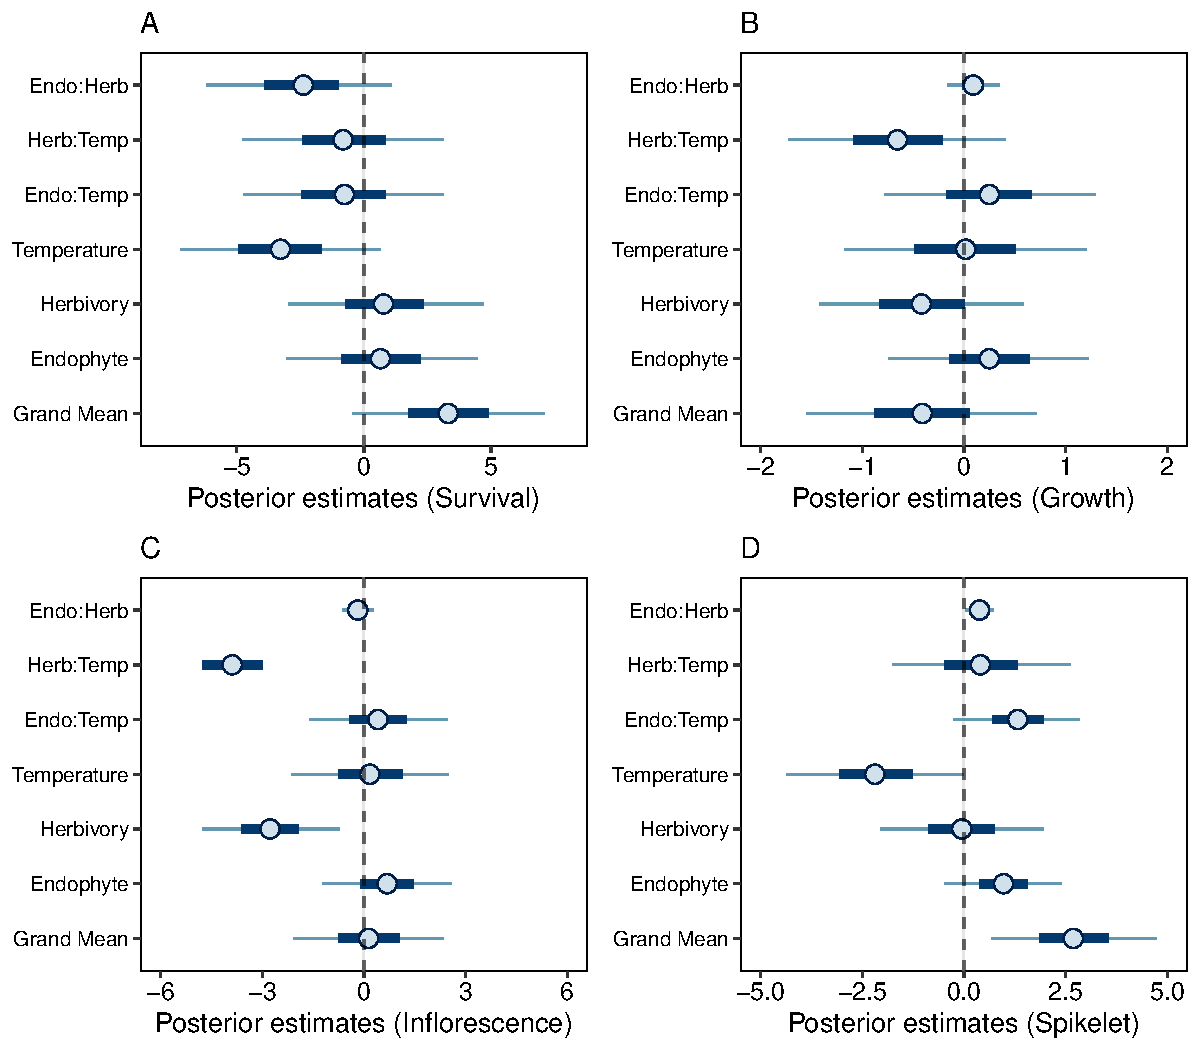
\includegraphics[width=1\textwidth]{Posterior_mean.pdf}
%\caption{Posterior mean estimates for each vital rate. 
%(a) Daily temperature, estimated from average hourly data collected by  HOBO data loggers. 
%(b) Daily  soil moisture, estimated  from average hourly data  collected by  HOBO data loggers. 
%}
%\label{fig:climate}
%\end{figure}
%
%\begin{figure}[H]
%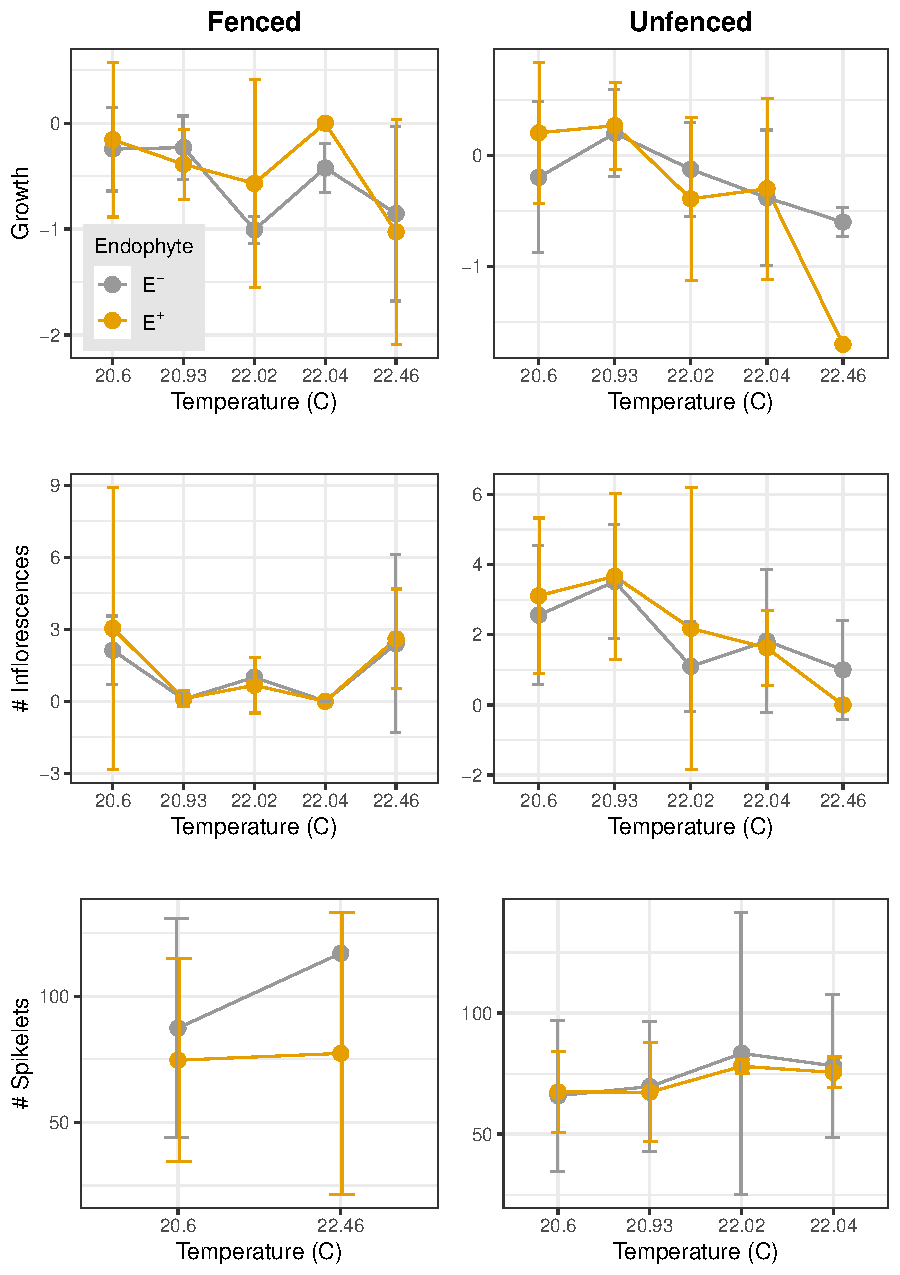
\includegraphics[width=0.9\textwidth]{Fig_temp_mean.pdf}
%\caption{Variation in vital rates across a temperature gradient.
%}
%\label{fig:vital}
%\end{figure}
%
%

\section*{Acknowledgements}
This research was supported by National Science Foundation Division of Environmental Biology awards 1543651 and 1754468 and by the Rice University Faculty Initiatives Fund.



\newpage
\bibliographystyle{apalike}
\bibliography{References}
%--------------------------------------------------------------------
\newpage
\clearpage 
\setcounter{equation}{0}
\setcounter{figure}{0}
\setcounter{section}{0}
\setcounter{table}{0}
\renewcommand{\theequation}{S.\arabic{equation}}
\renewcommand{\thetable}{S-\arabic{table}}
\renewcommand{\thefigure}{S-\arabic{figure}}
\renewcommand{\thesection}{S.\arabic{section}}

\centerline{\Large{\textbf{Supporting Information}}}
\subsection*{Study design}
\paragraph {Experimental Design} 
To understand the demographic effects of endophyte symbiosis from core to edge of the host range, we established  common gardens at 7 sites across the geographic range of \emph {Elymus virginicus} (Fig. \ref{sup:md}).
Experimental sites spanned an aridity gradient (temperature gradient).
Common gardens were established in 8 plots per site. 
Plots were 1.5m * 1.5m and the area was tilled of existing vegetation to control for native plant competition.
Plots were also selected in shaded areas under tree canopy or near shrubs to mimic the natural environmental of the species.
In each plot,  we planted 15 individuals  of \emph{E. virginicus} approximately 15 cm deep in an evenly spaced 4*4 grid pattern, with positions randomly assigned. 
For each plot, we randomly assigned a starting endophyte frequency  \jacob{(80\%, 60\%, 40\%, 20\%)}{Do we need a schematic of one replicate
of the experimental design?} and herbivory treatment (herbivores exclusion and herbivores accessibility). 
%Here, the endophyte frequency represents the percentage of  \emph{E. virginicus} individuals that have a symbiont ($E^+$).
We ensured that all plots had comparable quantities of source populations.
After establishing the plots, we watered the plants and recorded initial tiller counts, flowering status and plot position,  endophyte status, source population of each individual plant. 
For herbivory exclusion plots, we enclosed them with 1.2m tall mesh fencing to prevent browsing by vertebrate herbivores and sprayed the plots with insecticide. 
For herbivores accessibility plots (control treatment), we half enclosed the plots with the mesh netting.
%We stationed one HOBO MX2307 data logger at each site to collect temperature and volumetric water content in the soil every hour. 

\begin{figure}[H]
\centering
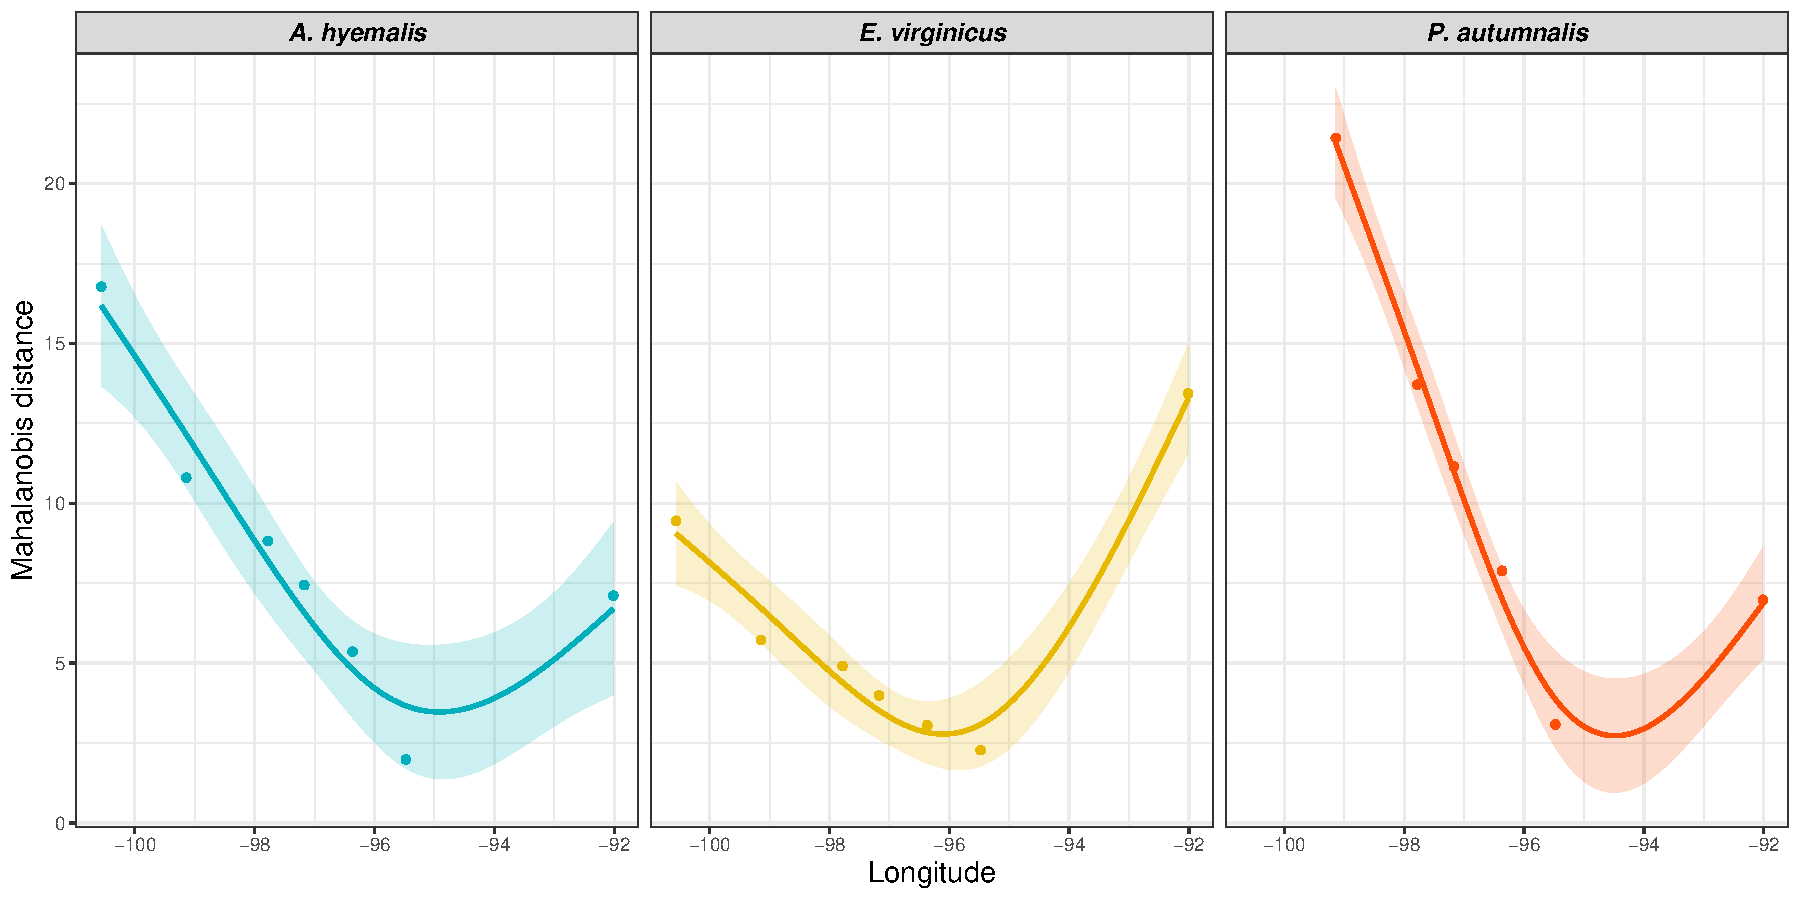
\includegraphics[width=1\textwidth]{distance_vs_longitude_gam.pdf}
\caption{Distribution of common garden sites along the longitudinal aridity gradient in the central and southern Great Plains for: A) Agrostis hyemalis, B) Elymus virginicus, and C) Poa autumnalis. Red dots indicate the locations of source populations, while grey dots represent GBIF occurrence records for each species within the study area. D) Relationship between the distance from the range center and longitude for each species.}
\label{sup:md}
\end{figure}


\paragraph {Source populations and Identification of individual endophyte status} 
Plants used  in the common garden experiment were derived from natural populations throughout the native range in the south-central US. 
At each of these natural populations we collected seeds. 
Some of the seeds of \emph{E. virginicus} were heat treated to produce endophyte negative plants ($E^-$) . 
To do so, we placed these seeds  in a drying oven set at 60°C for approximately five days (120 hours). 
While this method eliminates the endophytes from all individuals, it does not affect seed viability. 
All seeds (both heat-treated and non-heat-treated) were planted in the Rice University greenhouse.
Seedlings were regularly fertilized every two weeks. 
The seedlings were then vegetatively propagated to produce enough individuals for your experiment (N = 840).
Before planting in the field, we confirmed the endophyte status ($E^+$ or $E^-$) of all  seedlings using either microscopy or an immunoblot assay. 
This was necessary due to the varying success of the heat treatment and differences in the prevalence of endophytes between the natural populations. 
Leaf tissues were stained with aniline blue lactic acid and viewed under a compound microscope at 200x-400x to identify fungal hyphae. 
The immunoblot assay (Phytoscreen field tiller endophyte detection kit, Agrinostics Ltd. Co.) uses monoclonal antibodies that target proteins of Epichloë spp. and chromagen to visually indicate presence or absence. Both methods yield similar detection rates.  

%\begin{table}[ht]
%\centering
%\caption{Populations and Coordinates}
%\begin{tabular}{|p{2in}|l|l|l|}
%\hline
%\textbf{Population} & \textbf{Location} & \textbf{Coordinates} & \textbf{NE+ / NE-} \\ \hline
%Sam Houston State University Field Station  & Huntsville, TX & 30°44'30.5"N, 95°28'28.2"W & NE+ = 39, NE- = 50 \\ \hline
%Texas Tech University  & Junction, TX & 30°28'18.2"N, 99°47'01.7"W & NE+ = 49, NE- = 83 \\ \hline
%Palmetto State Park  & Palmetto, TX & 29.591623, -97.584781 & NE+ = 250, NE- = 192 \\ \hline
%Jean Lafitte National Historical Park and Preserve  & Jean Lafitte, LA & 29.785105, -90.114933 & NE+ = 83, NE- = 94 \\ \hline
%\end{tabular}
%\end{table}

\begin{table}[H]
\caption{Model comparison by vital rate using ELPD differences. Best models are bolded.}
\centering
\begin{tabular}{|l|l|r|r|}
\hline
\textbf{Vital rate} & \textbf{Model} & \textbf{elpd\_diff} & \textbf{se\_diff} \\
\hline
Survival   & \textbf{model1} & \textbf{0.0}   & \textbf{0.0} \\
           & model2          & -1.0           & 1.5          \\
           & model3          & -1.0           & 1.5          \\
\hline
Growth     & \textbf{model3} & \textbf{0.0}   & \textbf{0.0} \\
           & model2          & -1.3           & 2.0          \\
           & model1          & -2.1           & 2.2          \\
\hline
Flowering  & \textbf{model2} & \textbf{0.0}   & \textbf{0.0} \\
           & model3          & 0.0            & 3.2          \\
           & model1          & -1.3           & 3.9          \\
%\hline
%Spikelet   & \textbf{model2} & \textbf{0.0}   & \textbf{0.0} \\
%           & model3          & -4.6           & 4.2          \\
%           & model1          & -6.4           & 5.3          \\
\hline
\end{tabular}
\label{tab:elpd_vital_rates}
\end{table}





%\section {Supporting Figures}
%
%\begin{figure}[H]
%		\centering
%		\includegraphics[width=0.95\linewidth]{Figures/fig_tas_past_present_future.pdf}
%		\caption{Temperature variation across the study sites from 1990 to 2100,
%		ds: Dormant season, dg: Growing season.}
%		\label{Sup:temp_variation}
%\end{figure}
%
%\begin{figure}[H]
%		\centering
%		\includegraphics[width=0.95\linewidth]{Figures/fig_pr_past_present_future.pdf}
%		\caption{Precipitation variation across the study sites from 1990 to 2100.
%		ds: Dormant season, dg: Growing season.}
%		\label{Sup:pr_variation}
%\end{figure}
%
%\begin{figure}[H]
%		\centering
%		\includegraphics[width=0.95\linewidth]{Figures/MIROC.pdf}
%		\caption{Past, Observed, present and future (MIROC Model) climate data across the study area.}
%		\label{Sup:projectionMIROC}
%\end{figure}
%
%\begin{figure}[H]
%		\centering
%		\includegraphics[width=0.99\linewidth]{Figures/ACCESS.pdf}
%		\caption{Past, Observed, present and future (ACCESS Model) climate data across the study area.}
%		\label{Sup:projectionACCESS}
%\end{figure}
%
%\begin{figure}[H]
%		\centering
%		\includegraphics[width=0.99\linewidth]{Figures/CESM1.pdf}
%		\caption{Past, Observed, present and future (CESM1 Model) climate data across the study area.}
%		\label{Sup:projectionCESM1}
%\end{figure}
%
%\begin{figure}[H]
%		\centering
%		\includegraphics[width=0.99\linewidth]{Figures/CMCC.pdf}
%		\caption{Past, Observed, present and future (CMCC Model) climate data across the study area.}
%		\label{Sup:projectionCMCC}
%\end{figure}
%
%\begin{figure}[H]
%		\centering
%		\includegraphics[width=0.959\linewidth]{Figures/site_year_weather.pdf}
%		\caption{Climate variation across the study sites during the monitoring period.}
%		\label{Sup:climate_variation}
%\end{figure}


\end{document}
